%% Nature Communications build (Article). Written 2026-09-11 against paper/nc_npjdm_venue_lock.md:
%% abstract <=150 words with no references or abbreviations; main text <=5,000 words excluding the
%% abstract, Methods, references and legends; <=10 display items; legends <=350 words; <=70 references;
%% Methods after the Discussion; TRIPOD-AI checklist in the Supplement. Every number here is one the
%% repository's result files state; paper/check_numbers.py will read this file once it is complete.
%%
%% EMBARGO. Nothing from the embargoed external cohort may appear here until its permission file
%% records permission. The external section below carries the public GEO cohorts only.

\documentclass[pdflatex,sn-nature]{sn-jnl}
%% Springer Nature LaTeX template, CGX house layout (Desktop/6kit/!latex_template/
%% Springer_Nature_LaTeX_Template_CGXstyle, copied 2026-09-28): 170 x 257 mm text block, lineno
%% package in the left margin, Nature numbered references (sn-nature.bst, loaded by the class).
%% ---------------------------------------------------------------------------
%% House layout for Springer Nature / Nature-portfolio submissions.
%%
%%   %% ---------------------------------------------------------------------------
%% House layout for Springer Nature / Nature-portfolio submissions.
%%
%%   %% ---------------------------------------------------------------------------
%% House layout for Springer Nature / Nature-portfolio submissions.
%%
%%   \input{sn-house-layout}        %% immediately after \documentclass
%%   ... \maketitle ...
%%   \linenumbers                   %% immediately after \maketitle
%%
%% Three settings, each with the measurement that chose it. Delete this file and
%% its two lines to return to the class's own layout; nothing else depends on it.
%% ---------------------------------------------------------------------------

%% 1. THE PAGE. The class loads geometry ITSELF, with text={31pc,194.25mm} on A4
%%    under sn-nature, so a second \usepackage{geometry} errors and the block has
%%    to be reset with \geometry instead.
%%
%%    A4 is 210 by 297 mm, so 170 by 257 leaves 20 mm on every side. Measured
%%    consequence rather than an aesthetic one: artwork authored at the venue's
%%    179 mm maximum and inserted at \textwidth is scaled by textwidth/179, which
%%    the class's own block makes 0.73 and this makes 0.950. A 7 pt label in the
%%    source therefore renders at about 5.11 pt under the class and 6.65 pt here,
%%    and 5.11 pt is below every legibility floor a venue states.
\geometry{textwidth=170mm, textheight=257mm, top=20mm, left=20mm,
          footskip=12mm, marginparsep=3mm, marginparwidth=8mm,
          bindingoffset=0mm}

%% 2. THE FOLIO. It is already bottom-centred by the class's \ps@headings and
%%    needs nothing. **Do not "fix" it with \pagestyle{plain}.** This class's
%%    plain style is
%%        \def\@oddfoot{\vbox to 18pt{...\hfil ddd\thepage\hfil}}
%%    which prints a literal "ddd" before every page number. Checked in
%%    sn-jnl.cls at line 870; the same bytes ship in the template and in every
%%    project copy taken from it.

%% 3. LINE NUMBERS. Use the lineno PACKAGE, not the class's own `lineno` option,
%%    and the reason is measured rather than stylistic.
%%
%%    The class option turns on `vruler` with
%%        \setvruler[12bp][1][1][3][1][1.18\textwidth][26pt][-7pt][0.99\textheight]
%%    which pads the counter to THREE digits and places it at 1.18\textwidth on
%%    odd pages. At the block above that lands the numerals at x = 203.0 mm on a
%%    210 mm page, measured from a compiled test, so a three-digit number clears
%%    the trim by about 0.7 mm and a fourth digit does not clear it at all. A
%%    manuscript of any length reaches four digits: the paper this file was
%%    extracted from runs to line 1500 over 28 pages.
%%
%%    The lineno package puts them in the left margin instead, measured at
%%    x = 13.7 mm against a text block starting at 20 mm, on every page and at
%%    every digit count. `mathlines` numbers display equations too. It must load
%%    before hyperref, which is why this file is input right after \documentclass.
\usepackage[mathlines]{lineno}

%% \linenumbers goes after \maketitle, not here, so the title block stays
%% unnumbered. Putting it in this file would number the authors and affiliations.
        %% immediately after \documentclass
%%   ... \maketitle ...
%%   \linenumbers                   %% immediately after \maketitle
%%
%% Three settings, each with the measurement that chose it. Delete this file and
%% its two lines to return to the class's own layout; nothing else depends on it.
%% ---------------------------------------------------------------------------

%% 1. THE PAGE. The class loads geometry ITSELF, with text={31pc,194.25mm} on A4
%%    under sn-nature, so a second \usepackage{geometry} errors and the block has
%%    to be reset with \geometry instead.
%%
%%    A4 is 210 by 297 mm, so 170 by 257 leaves 20 mm on every side. Measured
%%    consequence rather than an aesthetic one: artwork authored at the venue's
%%    179 mm maximum and inserted at \textwidth is scaled by textwidth/179, which
%%    the class's own block makes 0.73 and this makes 0.950. A 7 pt label in the
%%    source therefore renders at about 5.11 pt under the class and 6.65 pt here,
%%    and 5.11 pt is below every legibility floor a venue states.
\geometry{textwidth=170mm, textheight=257mm, top=20mm, left=20mm,
          footskip=12mm, marginparsep=3mm, marginparwidth=8mm,
          bindingoffset=0mm}

%% 2. THE FOLIO. It is already bottom-centred by the class's \ps@headings and
%%    needs nothing. **Do not "fix" it with \pagestyle{plain}.** This class's
%%    plain style is
%%        \def\@oddfoot{\vbox to 18pt{...\hfil ddd\thepage\hfil}}
%%    which prints a literal "ddd" before every page number. Checked in
%%    sn-jnl.cls at line 870; the same bytes ship in the template and in every
%%    project copy taken from it.

%% 3. LINE NUMBERS. Use the lineno PACKAGE, not the class's own `lineno` option,
%%    and the reason is measured rather than stylistic.
%%
%%    The class option turns on `vruler` with
%%        \setvruler[12bp][1][1][3][1][1.18\textwidth][26pt][-7pt][0.99\textheight]
%%    which pads the counter to THREE digits and places it at 1.18\textwidth on
%%    odd pages. At the block above that lands the numerals at x = 203.0 mm on a
%%    210 mm page, measured from a compiled test, so a three-digit number clears
%%    the trim by about 0.7 mm and a fourth digit does not clear it at all. A
%%    manuscript of any length reaches four digits: the paper this file was
%%    extracted from runs to line 1500 over 28 pages.
%%
%%    The lineno package puts them in the left margin instead, measured at
%%    x = 13.7 mm against a text block starting at 20 mm, on every page and at
%%    every digit count. `mathlines` numbers display equations too. It must load
%%    before hyperref, which is why this file is input right after \documentclass.
\usepackage[mathlines]{lineno}

%% \linenumbers goes after \maketitle, not here, so the title block stays
%% unnumbered. Putting it in this file would number the authors and affiliations.
        %% immediately after \documentclass
%%   ... \maketitle ...
%%   \linenumbers                   %% immediately after \maketitle
%%
%% Three settings, each with the measurement that chose it. Delete this file and
%% its two lines to return to the class's own layout; nothing else depends on it.
%% ---------------------------------------------------------------------------

%% 1. THE PAGE. The class loads geometry ITSELF, with text={31pc,194.25mm} on A4
%%    under sn-nature, so a second \usepackage{geometry} errors and the block has
%%    to be reset with \geometry instead.
%%
%%    A4 is 210 by 297 mm, so 170 by 257 leaves 20 mm on every side. Measured
%%    consequence rather than an aesthetic one: artwork authored at the venue's
%%    179 mm maximum and inserted at \textwidth is scaled by textwidth/179, which
%%    the class's own block makes 0.73 and this makes 0.950. A 7 pt label in the
%%    source therefore renders at about 5.11 pt under the class and 6.65 pt here,
%%    and 5.11 pt is below every legibility floor a venue states.
\geometry{textwidth=170mm, textheight=257mm, top=20mm, left=20mm,
          footskip=12mm, marginparsep=3mm, marginparwidth=8mm,
          bindingoffset=0mm}

%% 2. THE FOLIO. It is already bottom-centred by the class's \ps@headings and
%%    needs nothing. **Do not "fix" it with \pagestyle{plain}.** This class's
%%    plain style is
%%        \def\@oddfoot{\vbox to 18pt{...\hfil ddd\thepage\hfil}}
%%    which prints a literal "ddd" before every page number. Checked in
%%    sn-jnl.cls at line 870; the same bytes ship in the template and in every
%%    project copy taken from it.

%% 3. LINE NUMBERS. Use the lineno PACKAGE, not the class's own `lineno` option,
%%    and the reason is measured rather than stylistic.
%%
%%    The class option turns on `vruler` with
%%        \setvruler[12bp][1][1][3][1][1.18\textwidth][26pt][-7pt][0.99\textheight]
%%    which pads the counter to THREE digits and places it at 1.18\textwidth on
%%    odd pages. At the block above that lands the numerals at x = 203.0 mm on a
%%    210 mm page, measured from a compiled test, so a three-digit number clears
%%    the trim by about 0.7 mm and a fourth digit does not clear it at all. A
%%    manuscript of any length reaches four digits: the paper this file was
%%    extracted from runs to line 1500 over 28 pages.
%%
%%    The lineno package puts them in the left margin instead, measured at
%%    x = 13.7 mm against a text block starting at 20 mm, on every page and at
%%    every digit count. `mathlines` numbers display equations too. It must load
%%    before hyperref, which is why this file is input right after \documentclass.
\usepackage[mathlines]{lineno}

%% \linenumbers goes after \maketitle, not here, so the title block stays
%% unnumbered. Putting it in this file would number the authors and affiliations.

\usepackage{graphicx}
\usepackage{booktabs}
\usepackage{amsmath}
\usepackage{xcolor}
\raggedbottom

\newcommand{\TODO}[1]{\textcolor{red}{[TODO: #1]}}

\begin{document}

\title{Parameter-free multimodal fusion with ModRank and a corrected clinical reference for bladder cancer survival}

\author*[1]{\fnm{Guanxing} \sur{Chen}}\email{guanxing.chen@cityu-dg.edu.cn}
\affil*[1]{\orgname{City University of Hong Kong (Dongguan)}, \orgaddress{\city{Dongguan}, \country{China}}}

\abstract{Multimodal survival models for bladder cancer are ranked on one public benchmark against a
clinical reference built from tumour grade, which barely varies here.
Rebuilding it with pathologic stage raised its concordance from 0.566
to 0.664, above two of four published models on these folds, and more than halved the added value of
three multimodal models. We introduce ModRank, which fits one penalised Cox model per
modality and averages their ranks without fitting the combination. It reached 0.721, the highest
reported on this benchmark, without separating from two rerun competitors. It exceeded the corrected
reference in two of four other benchmark studies, and its two-modality form did not exceed stage
beyond the noise floor in three cohorts without histology. Here we show that clinical references for
these models need pathologic stage and that, across five studies, none of six fitted fusions
significantly improves on a combination with nothing to fit.}

\maketitle
\linenumbers

\section*{Introduction}

Bladder cancer causes more than 200,000 deaths a year worldwide~\citep{bray2024globocan}. For the
quarter of patients who present with muscle-invasive disease and are treated by radical cystectomy,
the pathologic stage of the specimen is the strongest routine predictor of what happens after
surgery, and it guides whether adjuvant treatment is considered and how closely the patient is
followed~\citep{witjes2021eau}. Stage is also a coarse instrument. Patients with the same pT3N0
disease receive the same recommendation yet can have very different outcomes, and the staging
variables in the pathology report do not separate them. Outcomes remain heterogeneous within stage.
Transcriptomic classes of muscle-invasive tumours differ markedly in survival and cut across
stage~\citep{kamoun2020consensus, robertson2017blca}, and no staging category encodes the morphology
of the resected tumour. A multimodal model should therefore add the prognostic information that stage
does not capture.

Multimodal deep learning seeks that information in the slide and the transcriptome together. Weakly
supervised aggregation over whole-slide tiles made slide-level prediction practical without region
annotation~\citep{lu2021clam, chen2024uni, ding2025titan}, and a family of models now fuses slide
tokens with pathway-level expression through attention, optimal transport or prototype
learning~\citep{chen2021mcat, xu2023motcat, jaume2024survpath, song2024mmp, zhang2024pibd,
eijpe2025dimaf}. Their progress on bladder cancer is measured largely on one benchmark, the five-fold
splits of disease-specific survival that SurvPath released for 359 patients of The Cancer Genome
Atlas~\citep{jaume2024survpath}. Two properties of that benchmark decide what its leaderboard can
mean.

The first is the clinical reference. A multimodal model's added value is its improvement over the
clinical reference, which sets the zero point of every comparison. The clinical baselines published
on this benchmark are built from age, sex and tumour grade~\citep{jaume2024survpath, song2024mmp,
eijpe2025dimaf}. Muscle-invasive urothelial carcinoma is almost uniformly high grade, and a covariate
that places almost every patient in one category can separate few of them, so a grade-based reference
understates what the clinic knows. Benchmarks of multi-omics survival models include stage in the
clinical reference~\citep{herrmann2021benchmark, wissel2023noise, wissel2025survboard}. An
influential earlier whole-slide study built its reference from grade~\citep{chen2022porpoise}.

The second is the sample size. Three hundred and fifty-nine patients with 113 deaths from the
disease make a small survival problem. The events-per-parameter reasoning behind current sample-size
guidance for prediction models argues against fitting tens of millions of parameters to
it~\citep{riley2020samplesize}.
A method built for this regime should spend its events where the signal is and none on the
combination.

Here we measure both properties and build a method around them. We show that rebuilding the
clinical reference with stage, from the benchmark's own files, raises its concordance from 0.5664 to
0.6637 and more than halves the added value of three multimodal constructions, two of them published
architectures. We then
introduce ModRank, which fits one penalised Cox model per modality over a frozen foundation-model
slide embedding, pathway-level transcriptomics and stage, and combines them by an equal-weight rank
average with no fitted parameter. Under a protocol frozen after development it reaches the highest concordance
reported on the benchmark, although it is not significantly different from the two competitors we
could rerun. Fitting the fusion on identical inputs does not significantly improve on it. In bladder a
concatenated model falls below it and learned weights come within the benchmark's resolution of it,
and across the benchmark's five studies none of six fitted fusions is significantly ahead of it. ModRank
holds its concordance when whole hospitals are held out and gives two-year risks calibrated in the
large, with a
gain in accuracy over the clinical model that this cohort cannot resolve. It does not exceed the
corrected reference in two of the benchmark's four other studies, and in three external cohorts
without histology its two-modality form does not exceed stage beyond the noise floor.

%% ============================================================================ RESULTS (chunk 2)
\section*{Results}

\subsection*{The benchmark's clinical reference omits pathologic stage}

We read every method paper reported on the bladder cohort of the benchmark. Eight of the eleven
could be read in full. Four report a clinical-variable baseline, all four build it from age, sex and
tumour grade, and none uses pathologic stage. The other four report no clinical baseline at all
(Supplementary Note~1 and Supplementary Table~1). The three papers that could not be read are
recorded as unverified. The reported bladder values are 0.519 and 0.570 concordance. Stage is not missing from
the data. It is a column of the files released with the benchmark, and it sits directly beside grade
in the split files of the highest-scoring published method on these folds~\citep{eijpe2025dimaf} (Fig.~\ref{fig:overview}a).

The mechanism reflects the grade distribution of muscle-invasive disease. In the clinical file released with the benchmark, the
only clinical source common to all five of its studies, grade takes two levels with 94.4\% of cases
in one of them (normalised entropy 0.311), against five levels and 0.665 for stage
(Fig.~\ref{fig:overview}d). We then rebuilt the clinical arm twice, changing only grade to stage,
from the incumbent's own split files, which the method reads and which record stage as four American
Joint Committee on Cancer (AJCC) groups over 357 valued cases. The grade construction reaches 0.5664 and the stage construction 0.6637, a
gap of +0.0972 (95\% confidence interval $[+0.047, +0.150]$, $p<0.001$, 6,000 case-resampling
replicates) on identical cases through an identical pipeline. The stage-based reference exceeds two of the four published entries on verified folds and five of all nine
(Fig.~\ref{fig:missing}a, Table~\ref{tab:published}). The same one-column swap raises the clinical
arm in all five studies the benchmark covers, by $+0.0408$ to $+0.2211$, and in two of the five the
interval excludes zero (Fig.~\ref{fig:missing}c). In two of them the released
files carry no usable grade, so there the comparison is with age and sex alone (Supplementary
Table~2). Outside the benchmark, stage outperformed grade as the clinical reference in all six
independent bladder cohorts that record both (1,175 patients), with intervals excluding zero in five. The largest gap, $+0.2532$, was in a muscle-invasive cohort in which
94.5\% of tumours share one grade (Supplementary Note~9 and Supplementary Table~14).

\subsection*{Constraints on a method at 359 patients}

Before designing a model we measured three properties of the regime. A ridge Cox model fitted to
pure noise and scored in-sample reaches 0.7474 concordance at sixteen parameters, so an in-sample
fit on this cohort says little about signal. A two-parameter fusion fitted on the held-out fold,
which no deployed model could have, improves on equal weighting by only $+0.008$ (0.7268 against
0.7191), and a 21-point weight sweep peaks at exactly equal weight. A fusion gated on
clinical risk loses to its own permuted-stratum control (0.7493 against 0.7502), and none of the seven
components designed on this evidence passed its pre-registered test (Supplementary Note~2,
Supplementary Table~3 and Supplementary Fig.~1). Re-splitting the
same patients 24 times moves a paired difference between arms by a standard deviation of 0.0073, and
twice that, 0.0145, is the margin a difference must exceed to be stable under re-partitioning
(Fig.~\ref{fig:regime}).

The three measurements point the same way, to estimation rather than the fusion as the binding
constraint.
ModRank therefore fits one ridge-penalised Cox model per modality on the training fold (a 768-dimensional
TITAN slide embedding~\citep{ding2025titan}, the benchmark's own 275 pathway groups, and age, sex
and pathologic stage), maps each out-of-fold score to its within-fold percentile, and takes the
equal-weight mean. It carries 1,049 downstream coefficients and fits nothing in the combination
(Fig.~\ref{fig:overview}b).

\subsection*{ModRank against rerun competitors and fitted fusion}

Under the protocol frozen after development and five leakage checks, ModRank reaches
0.7214 concordance (mean over five seeds, standard deviation 0.0043, Supplementary Table~4). This is
the highest value reported on
these folds and $+0.0424$ above the best entry whose folds we verified (Table~\ref{tab:published}).
The two competitors whose implementations run end to end were given the same clinical variables by
the same rank average. ModRank exceeds SurvPath by $+0.0338$ ($[-0.0053, +0.0727]$, $p=0.087$,
competitor averaged over five retrainings) and PIBD by $+0.0252$ ($[-0.0173, +0.0676]$, $p=0.238$),
with 1,049 parameters against 24.7 and 26.9 million. Neither margin is significant at this cohort
size, and we read the ordering against published values as descriptive (Fig.~\ref{fig:result}).

The central design choice, one model per modality and nothing fitted in the combination, can be
tested on identical inputs. On the same features, folds, seeds and
estimator (Fig.~\ref{fig:robust}a), a single ridge Cox on all three blocks concatenated reaches $0.6861 \pm 0.0064$, and
fusion weights learned on inner out-of-fold scores (stacking) reach $0.7108 \pm 0.0032$ with a
fixed ridge and $0.7147 \pm 0.0048$ with a tuned one. ModRank
exceeds the concatenation by $+0.0342$ ($[+0.0015, +0.0681]$, $p=0.041$), the stacking by
$+0.0097$ ($[-0.0067, +0.0263]$) and the tuned stacking by $+0.0055$ ($[-0.0071, +0.0180]$), paired
on the seed-averaged scores. Over the 24 random re-partitions on which the noise floor was
measured, ModRank exceeds the concatenation ($+0.0471 \pm 0.0151$), the stacking ($+0.0107 \pm 0.0062$)
and the clinical arm ($+0.0549 \pm 0.0082$) in 24 of 24 (Fig.~\ref{fig:robust}b). The sign count
measures stability under re-partitioning, not superiority. The mean margin over the stacking is
smaller than the bar of 0.0145 that re-partitioning sets, so the two are not separable on this cohort, while
the margin over the concatenation clears it. With whole tissue
source sites held out, so that no hospital contributes to both sides of any fold (33 sites, five
folds), ModRank holds 0.7204 while the stacking falls to 0.6855 and the concatenation to 0.6482
(pooled point estimates, Fig.~\ref{fig:robust}c).

Two further checks bound the result. ModRank reads a 2025 slide encoder that the competitors did not.
Given instead the tile features SurvPath itself consumed, ModRank reaches 0.7004, still above every
published entry, which places the encoder's contribution at 0.0220 on the seed both values share.
And the protocol's
pre-registered selection correction was mis-specified. It used the standard deviation of a paired
difference where the maximum-of-candidates correction needs that of a single candidate's score. The primary does not clear the bar of 0.7708 measured under an outcome-permuted null (Supplementary
Note~2).

\subsection*{Added value falls when the reference includes stage}

A clinical reference fixes the zero point of every claim about what histology and transcriptomics
add, so we measured how far the reference moves it. For three multimodal constructions (ModRank, and
SurvPath and PIBD each given the clinical block), we computed the added value over each reference,
$C(\text{model} + \text{reference}) - C(\text{reference})$, and the inflation $D$, the difference
between the added value over grade and over stage.

Against the grade-based reference every construction appears to add substantially, $+0.1225$
($[+0.0695, +0.1733]$) for ModRank, $+0.0656$ for SurvPath and $+0.0842$ for PIBD. Against the stage-based
reference the added values fall to $+0.0588$, $+0.0249$ and $+0.0336$
(Fig.~\ref{fig:added}a), so $D$ is $+0.0637$, $+0.0407$ and $+0.0506$. Against the
stage-based reference, only ModRank's added value has an interval that excludes zero. That comparison
does not survive correction across the six prespecified comparisons (Holm $q=0.067$), so its
direction is suggestive rather than resolved.

Part of this difference comes from the combination rule. An equal-weight rank average dilutes a strong reference more than a
weak one, so a score that carries no information, combined in the same way, has $D = +0.029$ on
average and $+0.0416$ in ModRank's three-arm form (Methods). Against this benchmark the excess is
$+0.0214$ ($[+0.0050, +0.0388]$) for ModRank, $+0.0235$ ($[+0.0072, +0.0404]$) for PIBD and
$+0.0104$ ($[-0.0047, +0.0261]$) for SurvPath (Fig.~\ref{fig:added}b). Four further architectures
from the SurvPath code base, rerun on the same folds, reach 0.52 to 0.60 on their own. Three have
$D$ of $+0.030$ to $+0.033$, no more than the benchmark. The fourth, DeepMISL, returned one risk per
validation fold in 13 of its 25 retraining--fold pairs, which leaves the reference's ordering
unchanged, so its $D$ is $+0.005$ (Supplementary Note~8 and Supplementary Tables~12 and~13). The gap between the two references therefore mixes a property of the rule with an excess
that only a model carrying signal shows. $D$ was specified after the
confirmatory run, and its benchmark after the results in this paragraph were known.

\subsection*{Calibration and clinical utility}

ModRank emits a rank, so absolute risk has to be learned on top of it without touching a validation
outcome. Inside each training fold we fitted one Cox coefficient on the training cases'
inner-out-of-fold ModRank score and a Breslow baseline hazard, and applied both to the validation
cases. The clinical model received the identical treatment. Pooled over the validation folds, the
mean predicted two-year risk of death from the disease was 0.342 against an observed 0.341, the
calibration slope was 0.771 (clinical model 0.848), and predicted and observed risks agreed across
quintiles (Fig.~\ref{fig:added}c, Supplementary Note~6 and Supplementary Table~10). Against a
training-fold Kaplan--Meier null, the index of
prediction accuracy was 0.098 at one year and 0.151 at two years for ModRank, against 0.047 and 0.079
for the clinical model, and the two were equal at three years (0.105). Resampling patients with the
predictions held fixed, the two-year difference of $+0.0724$ has a 95\% interval of
$[-0.0056, +0.1504]$. At two years the point estimate of ModRank's net benefit exceeded both the
clinical model and treating everyone at every threshold examined from 20 to 60\%, for example 0.138 against 0.090 and $-0.098$ at
40\% (Fig.~\ref{fig:added}d). At 40\% the difference from the clinical model is $+0.0474$
($[+0.0040, +0.0907]$), and at the other four thresholds tested its interval includes zero, so the
utility gain is suggestive rather than established.

\subsection*{The method on the benchmark's other four studies}

The benchmark releases five studies and every method paper reports all five, so the four
non-bladder studies were scored with the identical recipe. They are not an independent test, because
an earlier form of the recipe was scored on them during development (Methods).
This protocol departs from the bladder primary in two ways. The clinical variables come from the
benchmark's own clinical file instead of the incumbent's split files, and the penalty is chosen once
rather than averaged over five seeds. Under it bladder reaches 0.7003, against 0.7214 under the
primary protocol. Every interval is a paired case-level bootstrap interval, as elsewhere in this
work.

Across 2,241 patients and 411 events, the recipe exceeds the corrected clinical reference in three
of the five studies by a margin whose interval excludes zero. In bladder the margin is $+0.0784$
($[+0.0298, +0.1267]$, $p=0.001$). In breast it is $+0.1201$ ($[+0.0519, +0.1897]$, $p<0.001$), and
in head and neck $+0.0725$ ($[+0.0206, +0.1231]$, $p=0.008$), shown in
Fig.~\ref{fig:validation}a. In the other two studies it does not. Stomach reaches $+0.0452$
($[-0.0155, +0.1070]$) and colorectal $+0.0231$ ($[-0.0701, +0.1192]$), the study with 37 events and
an interval 0.19 wide.

Each margin was also read against the noise its own study generates, by re-partitioning that study
24 times as the bladder floor was built. The paired difference is positive in every one of the 24
partitions in all five studies, and exceeds twice the re-partition standard deviation in four of
them. Colorectal is the exception, $+0.0238$ against a bar of 0.0267. In stomach the two criteria
disagree. Its margin clears the bar, $+0.0449$ against 0.0325, while its bootstrap interval covers
zero, so resampling the patients leaves the margin uncertain and re-partitioning them does not.

Because the slide arm rests on one pretrained encoder, the five studies were scored again with a
different one, a self-supervised model trained by another group, with the folds, the clinical block,
the transcriptome arm, the estimator and the bootstrap held fixed, on the patients it covers (all but
nine of the 2,241). Concordance falls in the three
studies that separate and rises slightly in the two that do not. The same three still separate from
the clinical reference: $+0.0574$ ($[+0.0044, +0.1101]$) in bladder, $+0.0849$
($[+0.0163, +0.1531]$) in breast and $+0.0576$ ($[+0.0070, +0.1094]$) in head and neck, with stomach
and colorectal again covering zero. Which studies separate does not depend on which of the two
encoders is used. Every arm, every
paired difference, every floor and both encoders are in Supplementary Note~4 and Supplementary
Table~8.

Two further analyses bound what these studies show. Substituting grade for stage inside the same
three-modality arm lowers it in all five studies, but only in colorectal does the interval exclude
zero, at $+0.0894$ with an interval of $[+0.0437, +0.1429]$ (Fig.~\ref{fig:validation}b). The clinical block's
contribution beyond the slide and transcriptome is not resolved in any study. The paired difference
between the three-modality and two-modality arms has an interval covering zero in all five, and its
point estimate is negative in breast ($-0.0232$, $[-0.0749, +0.0277]$). What these studies establish is that the
method can exceed a stage-based clinical reference outside the bladder cohort, as it does
in two of the four other studies, not that a third modality is necessary to it.

Every ModRank value here exceeds the value SurvPath reports on these same released folds. PIBD, whose released split files
are the same, reports higher values in the four other studies (0.736 in breast, 0.768 in colorectal,
0.640 in head and neck and 0.684 in stomach), so ModRank is above the best value published on this
partition only in bladder. Values published under any protocol are far higher
outside bladder. Under other protocols 0.794 for breast and 0.832 for colorectal have
been reported, against 0.6881 and 0.7140 here (Fig.~\ref{fig:validation}c).

The fusion alternatives were built on all five studies as well, because the claim about fitting the
combination had rested on the development cohort alone. A concatenated Cox and a stacked Cox
were scored against the rank average in each study, and none of the ten comparisons has an interval
that excludes zero in either direction. Four further fitted fusions, specified afterwards, fared the
same in all five studies (20 comparisons, none separating). They choose the arms' weights or the
stacking's ridge by inner cross-validation, add pairwise products of the arms to the stacking, or
weight the arms by tertile of clinical risk. The concatenation and the stacking trail the rank average by point estimate in
four studies and lead it in breast, where the concatenated model reaches 0.7578 against 0.6881
($-0.0696$, $[-0.1399, +0.0010]$, $p=0.054$). A correct clinical reference changes
concordance by $+0.0972$ ($[+0.047, +0.150]$), which separates, whereas no difference between the
fusion rules tested separates at these sample sizes (Supplementary Table~7).

\subsection*{The slide's contribution}

The slide and clinical scores are weakly correlated (Spearman 0.2443), as are SurvPath's joint
score and the clinical score (0.1927). The slide score separates patients where the clinical model
cannot. On the 5\% of comparable pairs that the
clinical model places closest together (1,211 of 24,219), the clinical arm is at chance (0.4975) and
the slide arm reaches 0.6214 (Fig.~\ref{fig:modalities}d and Supplementary Table~5). On the 3,892
pairs that neither the
transcriptome arm nor the clinical model separates, each placing the two patients within its closest
40\%, the slide arm reaches 0.6193 while those two arms sit at 0.5540 and 0.5633.

Each modality's contribution to the combination is less well resolved than its restricted-pair
behaviour. Removing one arm at a time from the three-modality average changes concordance by
$-0.0221$ for the slide ($[-0.0484, +0.0039]$, $p=0.097$), $-0.0224$ for the transcriptome
($[-0.0495, +0.0055]$, $p=0.107$) and $-0.0390$ for the clinical block ($[-0.0696, -0.0086]$,
$p=0.011$), so at this size only the clinical arm's removal is separable from zero
(Fig.~\ref{fig:result}e). The restricted pairs above suggest that the slide and the transcriptome
each carry information, but the cohort cannot establish that either is individually necessary to the
average.

The slide and transcriptome arms track different biology. The transcriptome arm tracks the basal, luminal and epithelial--mesenchymal axes (Spearman
0.3601, $-0.372$ and 0.3673). The slide arm's correlation with any of the eight standard axes is at
most 0.2236 in magnitude, and its two strongest pathway correlates are metabolic
(Supplementary Note~3 and Supplementary Fig.~2). Across the median split of the
basal-minus-luminal axis, the slide and clinical arms exchange places while ModRank moves far less
(0.7109 in the basal-leaning half and 0.6983 in the luminal-leaning half, Supplementary Table~6 and
Supplementary Fig.~3). Supplementary Figs.~4 and~5
draw the three modalities against one patient ordering and the pre-specified case series with its
histology.

\subsection*{External cohorts}

The benchmark has no held-out bladder cohort, so we tested the reference inflation and the
combination rule in independent public bladder cohorts under protocols fixed before their outcomes
were analysed. No public cohort we found records slides, survival and bulk
expression for the same patients (Methods), so these tests concern the transcriptome and clinical arms. The recipe was refitted inside each cohort by repeated cross-validation.

In the two cohorts that record grade, the transcriptome again added more over a grade-based reference
than over a stage-based one. In a Swedish cohort of 224 patients with 25 deaths from the
disease~\citep{sjodahl2012molecular}, where grade and stage both vary, $D = +0.0586$ ($[+0.0179,
+0.0984]$, $p=0.009$). The protocol tested $D$ against zero, but under this combination rule a score
without information also has a positive $D$, $+0.0197$ in this cohort. Against that benchmark,
computed after the protocol's analyses, the transcriptome's excess was $+0.0397$ ($[+0.0011,
+0.0780]$, $p=0.045$). In a cystectomy cohort of 93 patients with 38
deaths~\citep{riester2012combination}, $D$ was $+0.0324$ against $+0.0149$ for a score without
information, and the excess was not resolved ($+0.0093$, $[-0.0211, +0.0390]$). The protocol's
sensitivity analysis in that cohort, which excludes the three patients given chemotherapy before
cystectomy, gave $D = +0.1081$ ($[+0.0404, +0.1757]$). Three patients moving it this far make it fragile,
and the all-patient value is primary.

The combination rule did not replicate beyond each cohort's noise floor. The two-arm ModRank had the
best point estimate in the Swedish cohort (0.8792 against 0.8672 for the stage block and 0.8748 for
stacking) and in a third cohort of 73 patients~\citep{choi2014identification} (0.6389 against 0.6334).
In the Swedish cohort it also exceeded the transcriptome alone and the concatenation after Holm
correction ($p=0.003$ and $p=0.006$). But it did not exceed the clinical stage block by more than the
pre-registered bar in any cohort. In the cystectomy cohort, microarray pathway
scores were uninformative (0.4747), and the equal-weight average fell below the stage block (0.5896
against 0.6591). A variant that admits an arm only when it clears a permutation null inside the
training fold, defined before any of these cohorts was downloaded and added by a dated amendment
after the cystectomy results had been read, was tested only on the two cohorts not yet seen. It equalled ModRank where both arms were informative, fell below both the stage
block and ModRank (0.6170 against 0.6334 and 0.6389) where the transcriptome arm was weak, and
cleared the bar in neither cohort (Supplementary Note~5 and Supplementary Table~9).

%% ============================================================================ DISPLAY ITEMS
\begin{figure}[p]
\centering
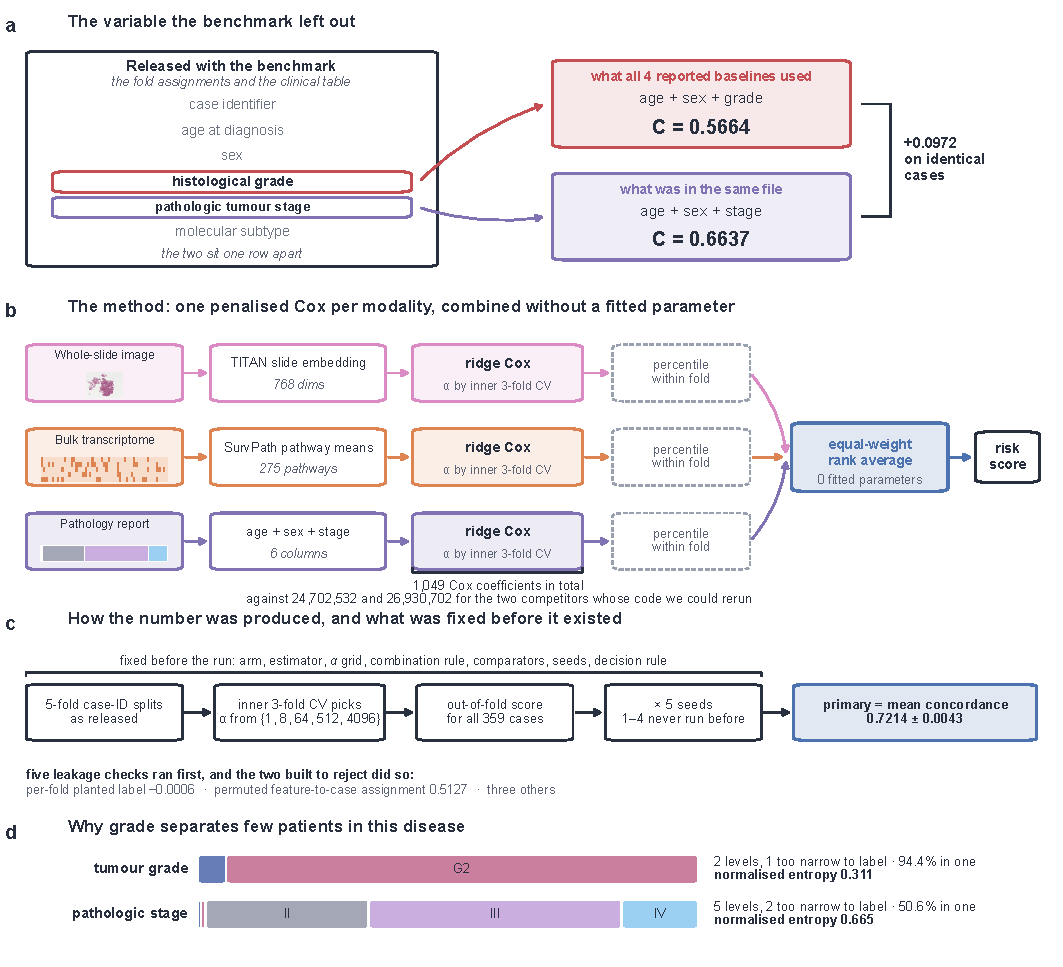
\includegraphics[width=\textwidth]{../figures/nc/fig1_overview.pdf}
\caption{\textbf{The clinical reference, the method and the protocol.} \textbf{a},~The files
released with the benchmark carry histological grade and pathologic tumour stage (American Joint
Committee on Cancer, AJCC) side by side. Every method paper we could read that reports a clinical
baseline builds it from grade. A clinical model with stage reaches 0.6637, against 0.5664 with grade,
on identical patients through an identical pipeline. \textbf{b},~ModRank fits one penalised Cox
model per modality to a frozen (not fine-tuned) slide embedding, pathway-level transcriptomics and
the staging variables, and combines them by an equal-weight rank average. It has 1,049
coefficients, against 24.7 and 26.9 million parameters for the two competitors whose code could be
rerun. The transcriptome glyph lights the 58 of 275 pathway groups whose correlation with the slide
arm has a Benjamini--Hochberg $q<0.05$. \textbf{c},~The choices the protocol fixed before the
confirmatory run. \textbf{d},~Why grade separates few patients here, in the clinical file released
with the benchmark. Grade has two levels, one holding 94.4\% of patients (normalised Shannon entropy
0.311), and stage has five (entropy 0.665). The models in \textbf{a} use the incumbent's split files
instead, where stage has four AJCC groups, drawn in Fig.~\ref{fig:modalities}a.}
\label{fig:overview}
\end{figure}

\begin{figure}[p]
\centering
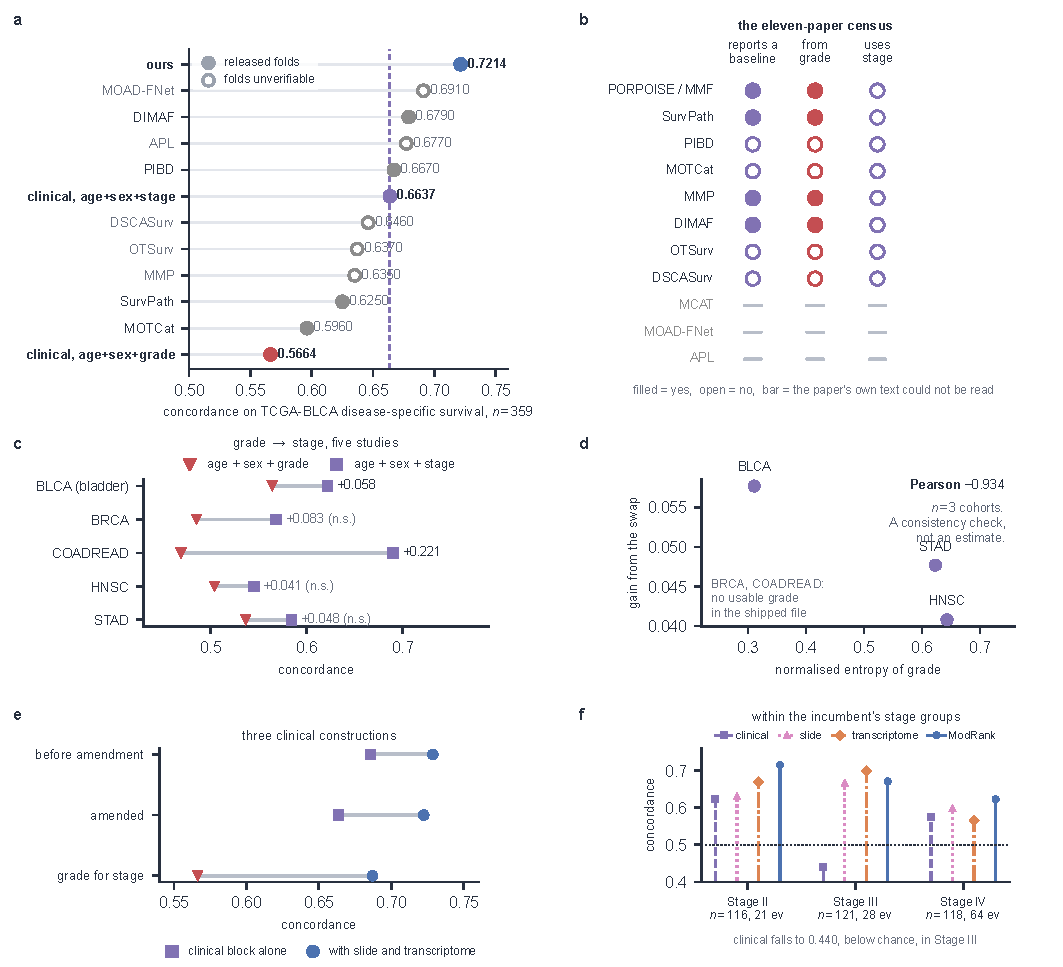
\includegraphics[width=\textwidth]{../figures/nc/fig2_missing_variable.pdf}
\caption{\textbf{The missing variable, quantified.} \textbf{a},~The nine published entries, ModRank
and the two clinical constructions. The dashed line marks the stage-based clinical arm. Two of the
four published entries on verified folds fall below it, and five of all nine. Entries whose folds
could not be verified are drawn open. \textbf{b},~The census, one row per paper. Four of the eight papers whose text could be read report a
clinical baseline, all four build it from grade, and none of the eight uses stage. The three that
could not be read are marked with a bar, not an inferred entry. \textbf{c},~The same one-column swap
in the five studies the benchmark covers, each on its own patients. The studies are bladder (BLCA),
breast (BRCA), colorectal (COADREAD), head and neck (HNSC) and stomach (STAD). In breast and colorectal the files
carry no usable grade, and the comparison is with age and sex alone. \textbf{d},~The gain is largest
where grade is least informative, across the three studies with a usable grade.
\textbf{e},~Three constructions of the clinical block, alone and with the other two modalities.
\textbf{f},~Within each stage group of the incumbent's split files (116, 121 and 118 patients), the
slide and transcriptome arms still separate patients.}
\label{fig:missing}
\end{figure}


\begin{figure}[p]
\centering
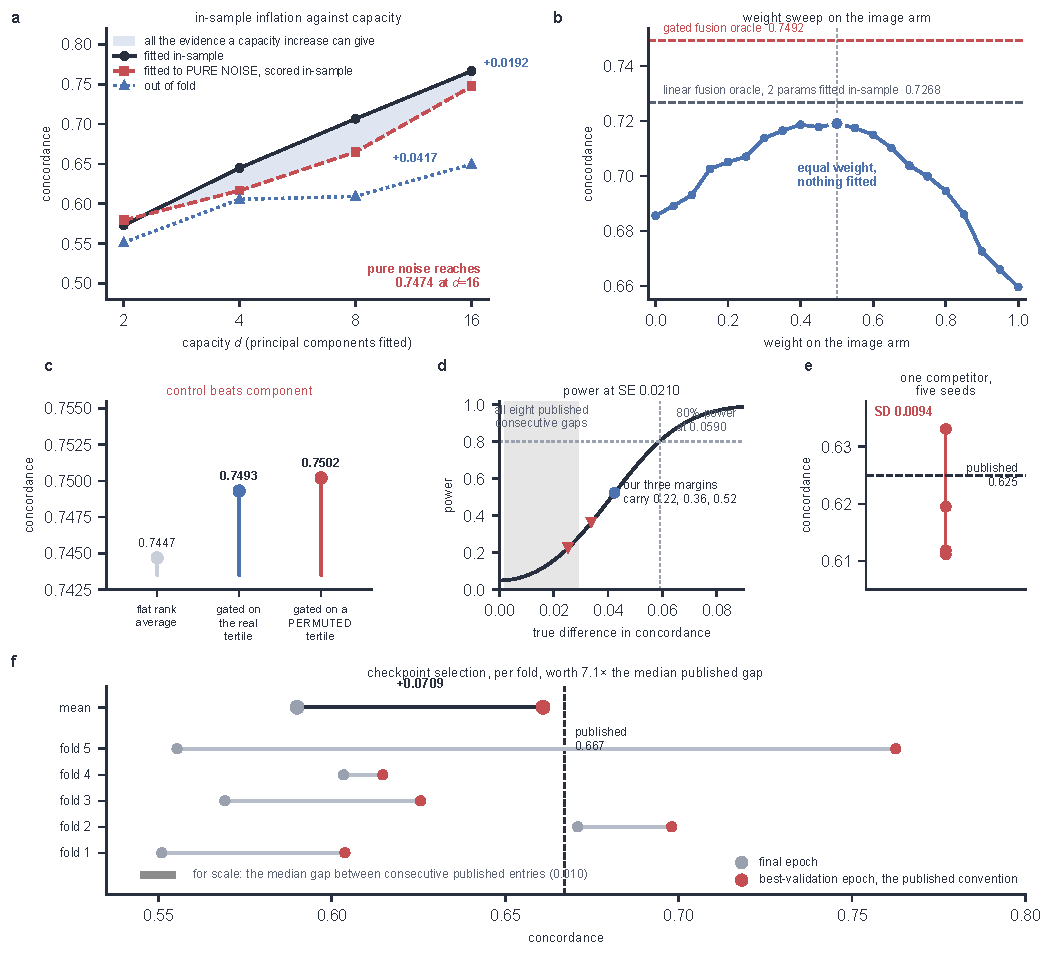
\includegraphics[width=\textwidth]{../figures/nc/fig4_regime.pdf}
\caption{\textbf{Constraints on a method at 359 patients and 113 events.} \textbf{a},~A ridge Cox model
fitted to pure noise and scored in-sample reaches 0.7474 at sixteen parameters. \textbf{b},~A 21-point weight sweep peaks at exactly equal weight, beside linear and gated fusions
fitted on the held-out fold, which no deployed model could have. \textbf{c},~A separate experiment,
a fusion gated on clinical risk inside the training fold, loses to its permuted-stratum control. \textbf{d},~Power of a paired comparison to detect a true
concordance difference, at this cohort's patient-resampling standard error. \textbf{e},~One
competitor across five retrainings. \textbf{f},~PIBD at the checkpoint selected on validation data and
at its final epoch, against the median gap between consecutive published entries.}
\label{fig:regime}
\end{figure}

\begin{figure}[p]
\centering
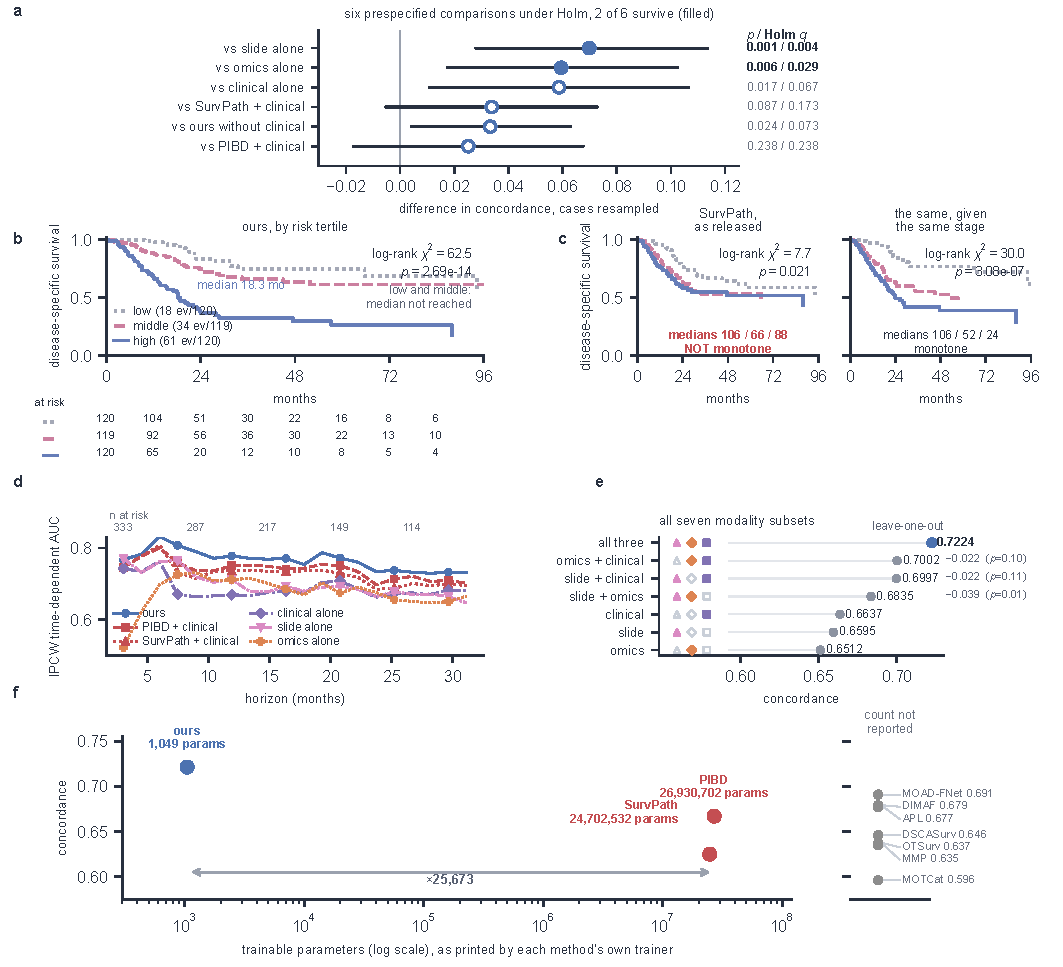
\includegraphics[width=\textwidth]{../figures/nc/fig3_method_result.pdf}
\caption{\textbf{The confirmatory result and the comparisons that do not survive correction.}
\textbf{a},~All six prespecified comparisons under Holm correction. Filled points survive at
$\alpha=0.05$ and open points do not. Both comparisons with the competitors given the same clinical
variables are among the four that do not, and the slide encoders differ between them.
\textbf{b},~Kaplan--Meier curves by risk tertile with the numbers at risk. \textbf{c},~SurvPath as
released, beside its predictions given the same clinical block. \textbf{d},~Time-dependent area
under the curve. \textbf{e},~All seven modality subsets at seed 0, with unadjusted intervals, so its comparison
without the clinical block is not the Holm-corrected one in \textbf{a}. \textbf{f},~Trainable parameters against
concordance. Two parameter counts are measured, and the other seven entries report none.}
\label{fig:result}
\end{figure}

\begin{figure}[p]
\centering
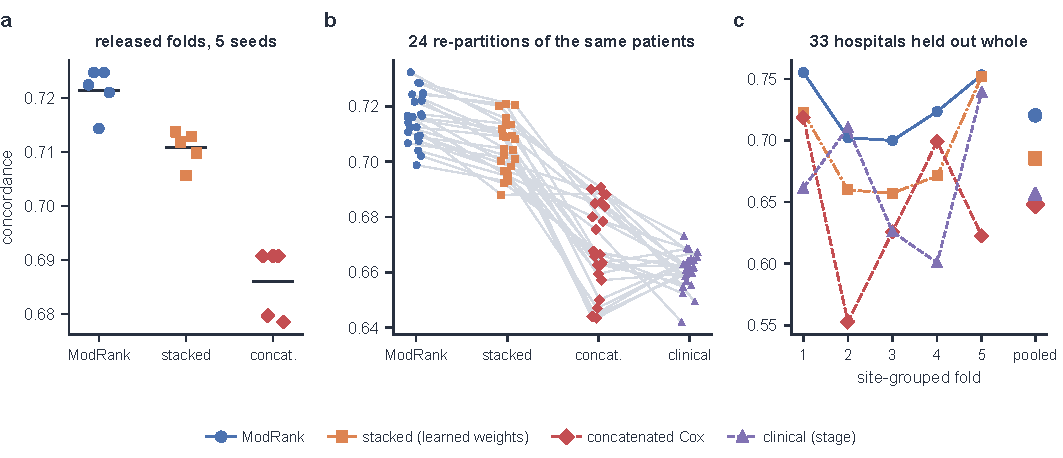
\includegraphics[width=\textwidth]{../figures/fig6_robustness.pdf}
\caption{\textbf{Fusion on identical inputs, and whether the ordering survives the partition.}
\textbf{a},~The released folds at five inner-cross-validation seeds (points, with the mean as a line). ModRank
($0.7214 \pm 0.0043$), weights learned on inner out-of-fold scores ($0.7108 \pm 0.0032$) and one
ridge Cox model on all three blocks concatenated ($0.6861 \pm 0.0064$) use the same features,
estimator and folds. \textbf{b},~The 24 random re-partitions on which the noise floor was measured.
Each grey line joins one partition's four values. ModRank is ahead of the stacking, the
concatenation and the clinical arm in 24 of 24. \textbf{c},~Five-fold cross-validation with whole
tissue source sites held out (33 sites), per fold and pooled. Pooled, ModRank reaches 0.7204, the
stacking 0.6855 and the concatenation 0.6482.}
\label{fig:robust}
\end{figure}

\begin{figure}[p]
\centering
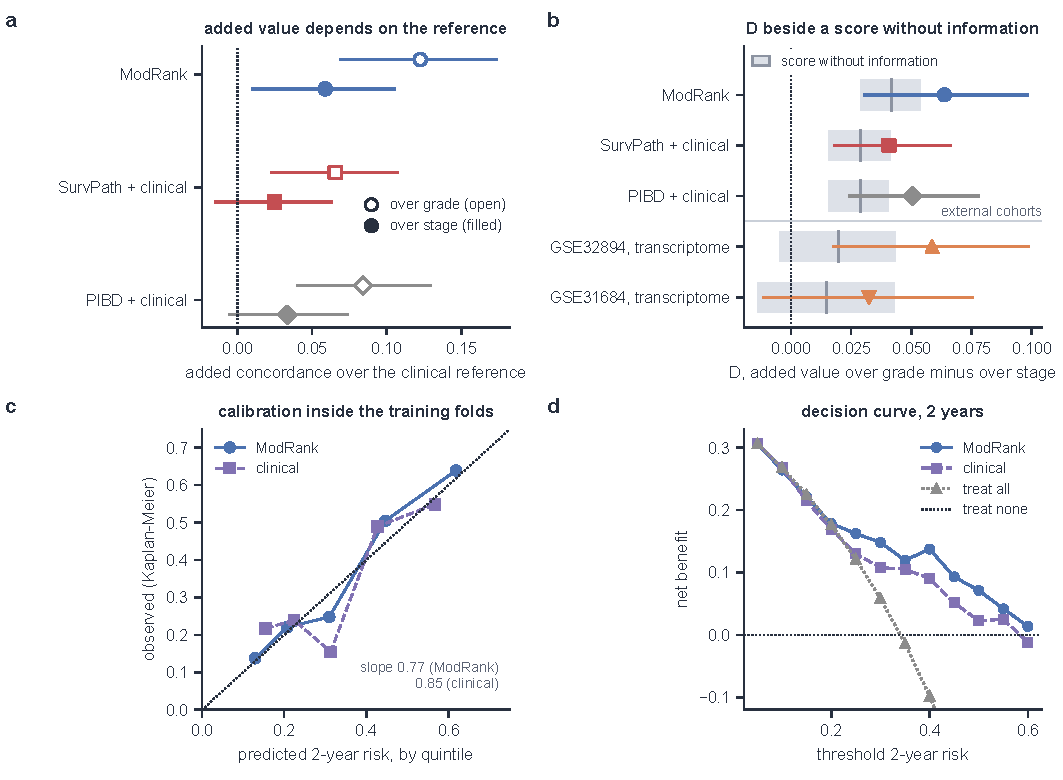
\includegraphics[width=\textwidth]{../figures/fig7_added_value_utility.pdf}
\caption{\textbf{Added value under two clinical references, and calibration and net benefit.} \textbf{a},~Added concordance over the grade-based (open) and the stage-based (filled)
reference for three multimodal constructions, with 95\% intervals from 6,000 patient resamples.
\textbf{b},~The inflation $D$, the added value over grade minus the added value over stage, in the
development cohort (three constructions) and in the two independent cohorts that record grade,
where the transcriptome is the added modality. Behind each estimate, the grey band spans the central
95\% of $D$ over 2,000 scores without information combined with the same references by the same rule,
and the grey line marks their mean. \textbf{c},~Two-year calibration by quintile of predicted risk,
with recalibration fitted inside the training folds only. The dotted line marks ideal calibration.
\textbf{d},~Net benefit at two years for ModRank, the clinical model, treating all and treating none.}
\label{fig:added}
\end{figure}

\begin{figure}[p]
\centering
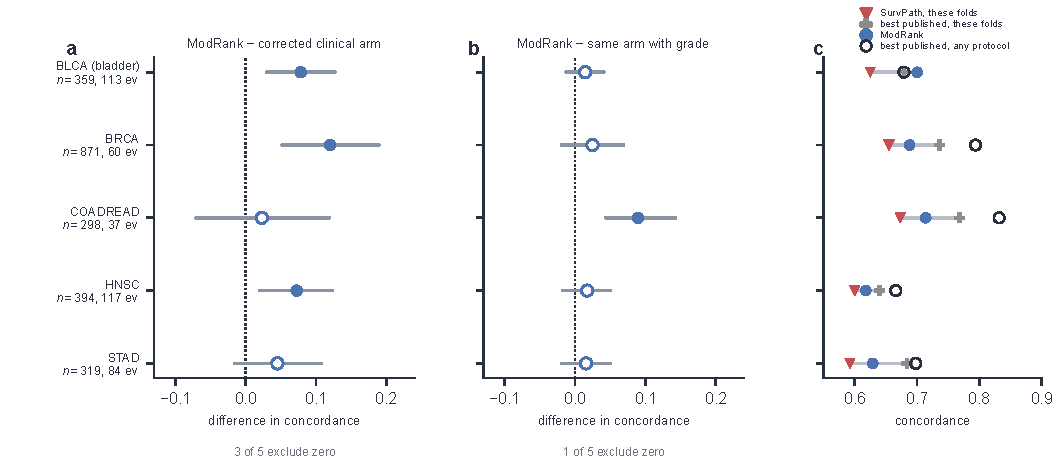
\includegraphics[width=\textwidth]{../figures/nc/fig8_five_cohort_validation.pdf}
\caption{\textbf{The same recipe on the benchmark's five studies, with intervals.} All 2,241
patients and 411 events, scored with the unchanged recipe on the released folds under the five-study
protocol (clinical variables from the benchmark's clinical file, one penalty selection), which gives
bladder 0.7003 against 0.7214 under the main protocol. Studies are bladder (BLCA), breast (BRCA),
colorectal (COADREAD), head and neck (HNSC) and stomach (STAD). Every interval is the 95\% interval
of a paired difference over 6,000 patient resamples. \textbf{a},~ModRank minus the corrected clinical
arm. Filled points mark an interval that excludes zero and open points one that does not, in the
same colour for all five studies. \textbf{b},~The same arm minus itself with grade
substituted for stage. \textbf{c},~Each study's ModRank value against three references: the value
SurvPath reports on these same released folds, the best value published on them (PIBD, which ships
the same split files, and DIMAF in bladder), and the best value published under any protocol,
which on BRCA and COADREAD lies far above every arm shown here.}
\label{fig:validation}
\end{figure}

\begin{figure}[p]
\centering
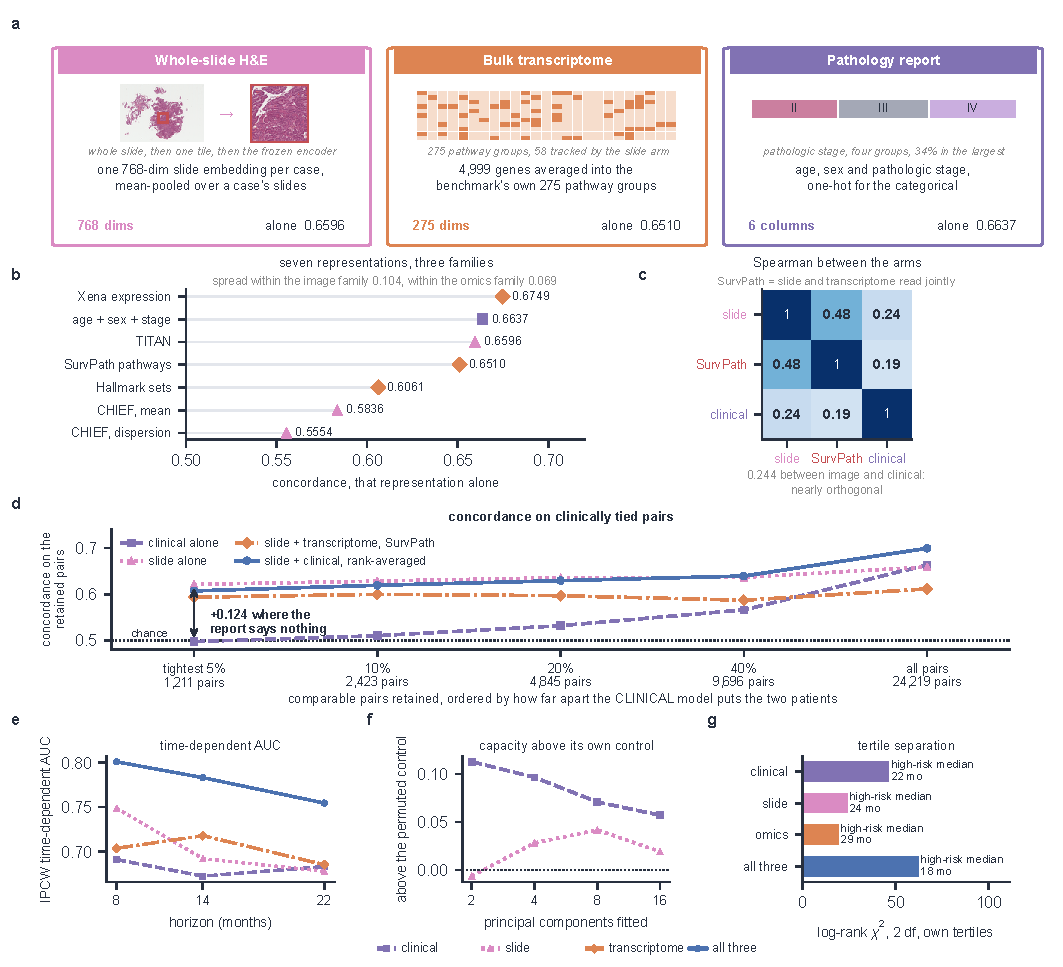
\includegraphics[width=\textwidth]{../figures/nc/fig3_modalities.pdf}
\caption{\textbf{The three modalities and the prognostic information each carries.} \textbf{a},~The inputs as they enter the model. All 359 patients carry all three. The histology is a diagnostic slide from
the study's own partition. \textbf{b},~Seven representations across the three families, on identical
patients and folds. \textbf{c},~Spearman correlation between the arms' out-of-fold scores, with the
amended clinical block. \textbf{d},~Comparable pairs restricted by the gap between the two
patients' clinical-model risk scores. On the tightest 1,211 of 24,219 pairs the clinical arm is at
chance (0.4975) and the slide arm reaches 0.6214. \textbf{e},~Time-dependent area under the curve at three horizons.
\textbf{f},~Concordance above the permuted control, by capacity. \textbf{g},~Log-rank separation across
each arm's own risk tertiles.}
\label{fig:modalities}
\end{figure}

\begin{table}[p]
\centering
\caption{Published concordance index values for disease-specific survival in the bladder cohort of
The Cancer Genome Atlas (TCGA) at $n=359$, with fold identity stated for each. The upper block uses
the released folds, verified here or by definition. The lower block used another or an unverifiable
protocol and is context only. Published values are as reported, which on these folds is generally
the mean of per-fold concordance, whereas ModRank's is pooled over out-of-fold predictions. On
ModRank's seed-averaged predictions the two conventions give 0.7276 and 0.7235.}
\label{tab:published}
\small
\begin{tabular}{llcl}
\toprule
method & venue & concordance & released folds \\
\midrule
\multicolumn{4}{l}{on the released folds, verified here or by definition} \\
ModRank (this work) & n/a & 0.7214 & verified (definitional) \\
DIMAF~\citep{eijpe2025dimaf} & MICCAI 2025 & 0.679 & verified, 5/5 folds identical \\
PIBD~\citep{zhang2024pibd} & ICLR 2024 & 0.667 & verified; rerun here at 0.6609 \\
SurvPath~\citep{jaume2024survpath} & CVPR 2024 & 0.625 & definitional \\
MOTCat~\citep{xu2023motcat} & ICCV 2023 & 0.596 & definitional (reported in SurvPath) \\
\midrule
\multicolumn{4}{l}{another or an unverifiable protocol, context only} \\
MOAD-FNet~\citep{moadfnet2024} & arXiv & 0.691 & unverified, no code released \\
APL~\citep{apl2025} & arXiv & 0.677 & unverified, repository empty \\
DSCASurv~\citep{song2025dscasurv} & Brief.\ Bioinform.\ 2025 & 0.646 & unverified \\
OTSurv~\citep{ren2025otsurv} & MICCAI 2025 & 0.637 & follows MMP's protocol \\
MMP~\citep{song2024mmp} & ICML 2024 & 0.635 & own site-stratified protocol \\
\bottomrule
\end{tabular}
\end{table}

\section*{Discussion}

Two findings concern how multimodal survival models for bladder cancer are measured, and one
concerns how they should be built. The benchmark's clinical reference omits pathologic stage, the
routine pathology variable that separates patients with muscle-invasive disease, and correcting it
more than halves what each of the three multimodal constructions we could measure appears to add
(Fig.~\ref{fig:added}). At 359 patients and 113 events, fitting the fusion on identical inputs does
not significantly improve on a method that fits nothing in its combination. The rank average has the
highest point estimate of the three constructions, ahead of learned weights by less than the
benchmark resolves and of concatenation by more. That ordering holds when the same patients are
re-partitioned and, in the pooled estimate, when whole hospitals are held out
(Fig.~\ref{fig:robust}).

The inflation is mostly a property of the reference rather than of the model. For each of three
constructions the gain over a grade-based reference is two to three times the gain over a
stage-based one. A score that carries no information, combined by the same rank rule, already shows
more than half of that difference, and four weaker architectures show no more. The remainder is an
excess that appears only with a model that carries signal. Its interval excludes zero for ModRank
and PIBD, for bladder under the five-study protocol and in the Swedish cohort, and not for SurvPath,
head and neck, stomach or the cystectomy cohort (Supplementary Note~8). In the external cohorts,
against the protocol's prediction, $D$ was larger where grade varied, so the determinants of the
excess are not settled.

Across the three benchmark studies with a usable grade, the gain from swapping grade for stage tracks
how uninformative grade is (Fig.~\ref{fig:missing}d). Across nine cohorts it does not (Spearman
$-0.07$), because stage outperformed grade in all nine, non-muscle-invasive cohorts included. Published comparisons are affected regardless. Two of the four published entries on verified folds, and five of all
nine, fall below a clinical model of age, sex and stage (Fig.~\ref{fig:missing}a), so a gain
reported over grade alone cannot be read as a gain over what the clinic knows. Multimodal survival
models for bladder cancer should report their added value over a clinical reference that contains
the stage available at the time of prediction, which for postoperative models such as these is
pathologic stage.

We propose a reason why the simplest combination holds its own here. The three modality scores are weakly correlated, each model is estimated from the events it can afford, and
nothing is estimated in the combination. Learned fusion spends events on weights, and a joint
penalised model spends them on 1,049 coefficients at once. On this cohort both fall below the rank
average in every one of 24 re-partitions, the stacking by a mean of 0.0107, which the benchmark
cannot resolve, and the concatenation by 0.0471, which it can. Holding out whole hospitals widens both gaps. Across the five
studies scored under one protocol, however, none of the six fitted fusions separates from the rank
average in either direction, and in breast the concatenation leads it by 0.0696 without separating. This is the
regime that sample-size guidance for prediction models anticipates~\citep{riley2020samplesize}.
With 113 events a method can afford few estimated quantities, and here spending them on the combination did not improve on
spending none.

The comparison with published entries supports a narrower claim. ModRank has the highest
concordance reported on these folds, but it cannot be distinguished from the two competitors that
could be rerun with the same clinical variables. Two corrections for having selected it set bars it does not reach, one measured under an
outcome-permuted null over the final family of 14 candidates and one for all 206 candidates under a
Gaussian approximation (Supplementary Note~2). Its net benefit over the
clinical model is suggestive, with an interval that excludes zero at one of five thresholds
(Fig.~\ref{fig:added}d). At this size the benchmark can separate a
stage-based clinical reference from a grade-based one, and it cannot rank methods whose
published values differ by a few hundredths.

The evidence that the method generalises is partial, and where it holds is informative. On the
benchmark's other four studies, which were consulted during development and are therefore reused
rather than independent, it exceeds a stage-based clinical reference in breast and in head and neck and does not in
stomach or colorectal (Fig.~\ref{fig:validation}a). The three-modality model is not separable from
its two-modality form in any of the five studies, so these cohorts show the method exceeding a correct
clinical reference rather than showing that a third modality is needed. Outside bladder it is below the
best value published on the same folds (Fig.~\ref{fig:validation}c).

External evidence bounds the method claim further. In three public cohorts without histology, the
two-arm form of the rule did not exceed the clinical stage block by more than each cohort's noise
floor, and where the microarray transcriptome carried no signal the equal-weight average fell below
the stage block (Supplementary Note~5). Fitting nothing in the combination has this cost, because an
uninformative arm dilutes the average. Admitting an arm only when it clears a permutation null did
not repair this where the transcriptome was weak, and no such screen can supply signal the arms lack.

The study has further limitations. The method was built on one public bladder cohort assembled
across many hospitals, retrospectively, with an endpoint derived from curated follow-up, and its
slide arm has not been tested outside it.
ModRank ranks a validation fold within itself, and a deployable variant that ranks each patient
against the training fold reaches 0.7245 against 0.7214, so within-fold ranking does not flatter the
result. Part of its lead over the published entries belongs to its slide encoder. Given the tile
features SurvPath consumed, it reaches 0.7004, still above every published entry. A
calibration slope of 0.771 indicates predictions that are too extreme and would be shrunk by
recalibration in a new setting. Performance by sex and age shows a limit of this cohort. Concordance
is lower in women than in men, for ModRank (0.6638 against 0.7399) and more so for the clinical arm
alone (0.5664 against 0.7014), but with 90 women and 31 events the bootstrap interval of the
difference between the sexes covers zero ($[-0.0244, +0.1844]$), and so does that of the difference
between the two arms' sex gaps. Above and below the median age the difference is small and its
interval covers zero. Race is absent from the benchmark's released files but recorded by the source
archive. Of the 359 patients, 285 are white, and no other category reaches the 25 patients and 100
comparable pairs required before a stratum is reported, so this cohort cannot support a comparison
between groups. Inside the white stratum ModRank still exceeds the clinical arm by
$+0.0594$ ($[+0.0052, +0.1134]$). No measure of socioeconomic position is recorded anywhere in these
data (Supplementary Note~7 and Supplementary Table~11).
Deployment would need a digitised diagnostic slide, tumour expression profiling and the pathologic
stage of the resected specimen, which is available only after surgery. Time is measured from initial pathologic diagnosis, although the inputs include
the stage of the resected specimen, so the model is not yet a risk estimate anchored at the
postoperative moment when a clinician would use it. A landmark analysis from the date of surgery would
be needed for that. Disease-specific survival also treats death from other causes as censoring in a
cohort whose median age is high. A competing-risk formulation would handle these deaths directly, and
we did not run one.

The practical recommendations do not depend on the leaderboard. Clinical references for multimodal
survival models in bladder cancer should include pathologic stage, added value should be reported
against that reference, and at the sample sizes public cohorts provide, a fusion rule with nothing to
fit is a strong baseline that learned fusion has to beat on identical inputs before its gain is
attributed to the architecture.

\section*{Methods}

\subsection*{Cohort, endpoint and prediction time point}

The development cohort is the bladder study of The Cancer Genome Atlas as partitioned by the
benchmark~\citep{jaume2024survpath}, 359 patients with both a diagnostic whole-slide image and a
disease-specific survival label, with 113 events and 24,219 comparable pairs. Time and event derive from
the Pan-Cancer Clinical Data Resource~\citep{liu2018tcgacdr}, which measures every endpoint from the
date of initial pathologic diagnosis. The tumours had not been exposed to chemotherapy when the
tissue was acquired~\citep{robertson2017blca}, and stage is the pathologic stage of the resected
specimen. The inputs are therefore available only after surgery, so a model built on them could
inform adjuvant treatment and follow-up once anchored at the date of surgery (Discussion), and cannot
inform the decision to give neoadjuvant chemotherapy, which precedes the specimen. The study uses
public, de-identified data only and required no ethical approval. Reporting follows the TRIPOD+AI
statement~\citep{collins2024tripodai} (Supplementary Table~17).

\subsection*{Folds, representations and estimator}

We used the benchmark's five released fold files unchanged and recorded their membership by hash in
the prespecified protocol. We verified fold identity for each comparator where a repository
allowed it. Entries on other or unverifiable protocols are reported as context only
(Table~\ref{tab:published}).

The slide representation is one 768-dimensional TITAN embedding per slide from a public precomputed
release~\citep{ding2025titan}, mean-pooled over a patient's slides. TITAN was pretrained without
patient outcomes and without TCGA slides. The transcriptome representation averages the benchmark's
4,999-gene matrix within the 275 of its 331 pathway groups that contain at least three of those genes.
The clinical block holds age, sex and AJCC pathologic tumour stage (one-hot) from the incumbent's
released split files, and the grade construction takes histological grade from the same files.
Missing levels enter as the reference level, and no patient is dropped.

Each arm is a ridge-penalised Cox model~\citep{cox1972regression, simon2011regularization} fitted by
limited-memory BFGS on the exact Breslow partial likelihood. The penalty is chosen from $\{1, 8, 64, 512, 4096\}$
by three-fold inner cross-validation inside the training fold, and standardisation uses
training-fold moments only. Out-of-fold linear predictors are mapped to within-fold percentiles, and
ModRank is the within-fold percentile of their equal-weight sum. A deployable variant that ranks a
new patient against the training fold's own scores reaches 0.7245 against the transductive 0.7214
(paired $p=0.59$).

\subsection*{Protocol, leakage checks and uncertainty}

The protocol fixed the arm, estimator, penalty grid, combination rule, comparator set, seeds and
decision rule after the development campaign and before the confirmatory run. Five leakage checks
came first. They tested fold integrity, the standardisation boundary by mutation, a per-fold planted
label, row permutation and outcome provenance, and the two built to reject did so. One amendment,
made after a cached query was found to have taken the first of several diagnosis records per patient,
rebuilt the clinical block from the incumbent's own files. Its effects, in opposite directions, moved
the primary from 0.7260 to 0.7212 (Supplementary Note~2). A second amendment corrected two
implementation defects found in review. The Cox fit had left out of each event's risk set the
patients who shared its time but were sorted before it, so it did not maximise the Breslow partial
likelihood the protocol specifies and depended on row order. Within-fold percentiles had broken
exact ties in the order of NumPy's default sort, which depends on the build. Every event now uses all
patients whose time is at least its own, and tied scores share their average rank. With nothing else
changed, every result after the confirmatory run was regenerated, which moved the primary to 0.7214
(Supplementary Note~10 and Supplementary Table~15). The development campaign and the confirmatory run
are reported as they were recorded.

Concordance is Harrell's~\citep{harrell1982cindex}, pooled over
out-of-fold predictions after within-fold percentile normalisation. The primary averages concordance
over five inner-cross-validation seeds. Paired comparisons use the seed-averaged score vector with
6,000 replicates that resample patients, never pairs. The intervals are conditional on the fitted
scores, which are not refitted in each replicate, and a difference reported with such an interval is
the mean of its replicates. The noise floor fixed by the protocol is the standard deviation, over 24
random re-partitions, of the paired difference between a rank-averaged arm and the clinical arm
(0.0073).

\subsection*{Fusion alternatives, re-partitions and held-out sites}

The concatenated model is one ridge Cox on all 1,049 columns with the penalty grid extended to
32,768. The stacked model fits three weights (ridge 1.0) on the inner
out-of-fold percentiles of the three arms inside each training fold and applies them to the
validation percentiles. Three further fusions, specified after the five-study results were known and
before they were run, use the same inner out-of-fold percentiles. The first chooses non-negative
weights summing to one from a grid of step 0.1 (66 points) by inner concordance. The second adds the
three pairwise products of arm percentiles to the stacked model. The third chooses such weights
separately within each tertile of the clinical arm's inner out-of-fold percentile and applies them by
the validation patient's clinical tertile. A fourth, added with the second amendment, is the stacked
model with its ridge chosen from $\{0.1, 1, 10, 100\}$ by three-fold cross-validation over the same
inner out-of-fold percentiles, on the inner split that produced them, so its tuning is not fully
nested. The re-partitions are the same 24 that define the noise floor. For the
site-grouped analysis, whole tissue source sites (the contributing institution, the second field of
the patient identifier) were assigned to five folds, largest first to the fold holding fewest
patients.

\subsection*{Added value and its inflation}

For a construction $M$ and a clinical reference $R$, the added value is $C(M+R)-C(R)$, where $M+R$
combines them by the same rank rule. The inflation is $D = [C(M+\text{grade}) - C(\text{grade})] -
[C(M+\text{stage}) - C(\text{stage})]$. All four concordances are recomputed on each of 6,000
patient resamples. Competitors' scores are their own released out-of-fold predictions: SurvPath
averaged over five retrainings, and PIBD at its best-validation checkpoint, the convention behind its
published value.

An equal-weight rank combination dilutes a stronger reference more, so $D$ is positive even for a
score that carries no information. Each $D$ is therefore compared with a benchmark that keeps the
reference and the combination rule and replaces the construction by random within-fold ranks, one
random arm for a two-arm construction and two for ModRank's three-arm sum. The benchmark's $D$ is its
mean over 2,000 random draws. The excess, $D$ minus that mean, has an interval from the same 6,000
resamples, on each of which the benchmark is averaged over 20 fixed random draws. In the external
cohorts the random arm replaces the transcriptome within each repeat of cross-validation. This
comparison was specified after the analyses it qualifies had been run.

The further architectures are MCAT~\citep{chen2021mcat}, ABMIL~\citep{ilse2018abmil},
TransMIL~\citep{shao2021transmil} and DeepMISL~\citep{yao2020deepattnmisl}, each with pathway
inputs. They were trained from the SurvPath code base on the released folds with the same tile
features and the settings of their released scripts, five times each, under a protocol committed
before they were run. MOTCat~\citep{xu2023motcat},
whose implementation that code base does not include, was not run.

\subsection*{Calibration and decision curves}

Within each training fold, a three-fold inner split scored the training patients with the same
construction. One Cox coefficient on that score and a Breslow baseline hazard were fitted and applied
to the validation patients to give survival at 12, 24 and 36 months. We report the calibration slope,
calibration in the large (mean predicted against Kaplan--Meier observed risk at each horizon),
grouped calibration, the inverse-probability-of-censoring weighted Brier score, the index of
prediction accuracy against a training-fold Kaplan--Meier null, and net benefit against treating all
and none, with the event rate among patients above each threshold estimated by Kaplan--Meier.

\subsection*{The other four studies of the benchmark}

The benchmark releases five studies. After the bladder protocol was fixed, the unchanged recipe was
applied on the released case-level folds of the other four. These studies were not unseen. Before
the freeze, an earlier form of the recipe, with slide and transcriptome arms and age and sex, was
scored on all four to ask whether a bladder result carried over, and a rejected candidate estimated a
slide-embedding prior from their 1,882 labelled cases. Their results are a reused-cohort evaluation
under a fixed protocol, not an independent confirmation. Slide features are the same pan-cancer embeddings,
the transcriptome arm the same pathway groups, and the clinical arm age, sex and one-hot pathologic
stage read from the clinical files released with the benchmark. Two deliberate departures from the
bladder primary are reported wherever these numbers appear. The clinical variables come from the
benchmark's released clinical file rather than the incumbent's split files, and inner
cross-validation selects the penalty once rather than at each of five seeds. With both departures,
bladder ModRank is 0.7003 against the primary's 0.7214. Intervals use the same paired case-level
bootstrap as everywhere else in this work, and each arm's point estimate was reproduced in every study
before any interval was computed. The pre-registered scope used these studies to replicate the
clinical-reference finding. On 2026-09-12, after the intervals were computed, an amendment extended it
to a test of the method, and records the three limits that remain.

\subsection*{External cohorts}

Three public cohorts were admitted by a count, made before any outcome was analysed, of expression,
stage, age, sex and a timed disease-specific outcome recorded for the same samples. Two of them also
record grade, which the inflation analysis needs. Three further series were excluded (a duplicate,
cell lines, and a cohort mixing patients given neoadjuvant chemotherapy). The analysis protocol, fixed
before any of their outcomes was analysed, specifies the endpoints, the clinical blocks, probe-to-gene
mapping by the platform annotation, the same pathway definitions with groups of at least three
mapped genes, five repeats of stratified five-fold cross-validation, and a noise floor from 24
re-partitions. A variant that admits an arm only when it clears a permutation null inside the training
fold was defined before any of these cohorts was downloaded, and an amendment added it before the
results of two of the three cohorts were inspected (Supplementary Note~5).

No public cohort we found records a diagnostic whole-slide image, bulk tumour expression and a timed
outcome for the same patients. The search, run in September 2026 under a plan written before it
began, covered 37 imaging, genomic, trial-sharing, general-purpose and challenge repositories, the 33
bladder expression cohorts with outcomes from an earlier systematic enumeration, and the literature
from 2019 to 2026 on slide-based models of bladder cancer outcome (Supplementary Note~11 and Supplementary Table~16). Several
portals could not be searched natively, so the result describes this search rather than every
archive. It found one challenge dataset whose rules bar publishing results before the organisers'
papers appear, on which we report nothing, and one trial cohort, SWOG S1314, in which slides and
expression exist for 180 patients who all received neoadjuvant chemotherapy and whose slides and
outcomes are released only on request to the trial group~\citep{flaig2021s1314,bai2025gmlf}. The
slide arm was therefore not evaluated outside the development cohort.

Four further cohorts were assembled for the reference comparison alone, which needs grade, stage and
an outcome but no expression. They were chosen by a systematic search of the Gene Expression Omnibus,
ArrayExpress and cBioPortal under a protocol written before any download. Each was admitted by a count,
made before any outcome was analysed, of at least 50 patients with grade, stage, a time and an event
indicator, at least 20 events, and two or more levels of both grade and stage. GSE19915,
E-MTAB-1803, GSE13507 and E-MTAB-4321 were admitted, and two series whose deposited files carry no time
or event field were not. The grade and stage models are fitted by the recipe above with age and sex
where the cohort records them, each cohort on its own endpoint. Before any new cohort was scored, the
same code reproduced the two earlier cohorts' stage-block and grade-block concordances
(Supplementary Note~9).

\subsection*{Software and use of language models}

Every ModRank analysis ran on CPU. The development campaign and the confirmatory run used Python
3.8.20, NumPy 1.24.4 and SciPy 1.10.1. The results regenerated under the second amendment used
Python 3.9.6, NumPy 2.0.2 and SciPy 1.13.1, and for the external cohorts Python 3.8.10, NumPy 1.24.2
and SciPy 1.8.1. The competitors' reruns used their own code on one GPU each. Large language
models were used for code implementation assistance and for copy-editing and polishing the manuscript.
All analyses, results and claims were designed, run and verified by the author.

\section*{Data availability}

All data are public. The benchmark's splits, pathway definitions and clinical files are those
released with SurvPath (\url{https://github.com/mahmoodlab/SurvPath}). TCGA bladder data are from
the Genomic Data Commons~\citep{heath2021gdc}. The external cohorts are from the Gene Expression
Omnibus (GSE31684, GSE32894, GSE48075, GSE19915~\citep{lindgren2010combined} and
GSE13507~\citep{kim2010progression, lee2010e2f1}) and ArrayExpress
(E-MTAB-1803~\citep{rebouissou2014egfr} and E-MTAB-4321~\citep{hedegaard2016uromol}). Source data are provided with this paper.

\section*{Code availability}

All analysis code, the prespecified protocols with their amendments, the record of every candidate
scored during development, the confirmatory run, the outcome-permuted selection null and the external
analyses are publicly available at \url{https://github.com/gxCaesar/modrank} and archived on Zenodo as
version 1.3.4 (\TODO{version DOI, written when the deposit is published}). All archived versions
resolve from \url{https://doi.org/10.5281/zenodo.22025756}. The archive includes a script that recomputes the
reported numbers from the deposited result files rather than reading them from this manuscript.

\bibliography{../references}

\section*{Acknowledgements}

The author thanks the developers of SurvPath and PIBD for releasing pipelines that could be rerun end
to end, and the developers of DIMAF for releasing the split files used to build the clinical block.
The results published here are in whole or part based upon data generated by the TCGA Research
Network (\url{https://www.cancer.gov/tcga}). The histology shown comes from the open-access tier of
the National Cancer Institute Genomic Data Commons. This work was supported by the Guangdong Basic and
Applied Basic Research Foundation (No.~2025A1515110446).

\section*{Author contributions}

G.C. conceived the study, designed and executed the analyses, and wrote the manuscript.

\section*{Competing interests}

The author declares no competing interests.


\end{document}
